\chapter{Design and Implementation}
\label{chap:implementation}
Figure \ref{fig:three-tier-architecture} gives an overview of the three-tier architecture of the jSCAPE system, the relationships between each of the main components, and some of the tasks that they perform. The student view is implemented as a JavaFX applet embedded into the web browser. It communicates with a custom written Java application server using a custom built communication protocol. Finally, the application server also connects to a PostgreSQL database, to perform the standard read and write operations. \newline

\begin{figure}[H]
\centering
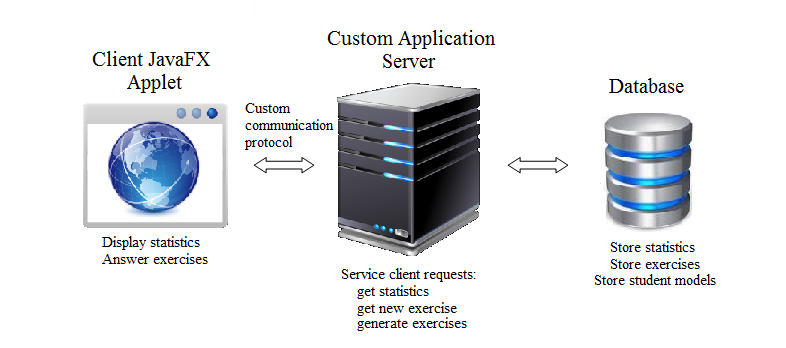
\includegraphics[width=\textwidth,height=\textheight,keepaspectratio]{three-tier-architecture}
\caption{Three tier architecture of the jSCAPE system.}
\label{fig:three-tier-architecture}
\end{figure}

The jSCAPE admin tool isn't really part of the core system's three tier architecture. The component was written later on to facilitate certain functions such as analyzing results and exercise bank management. To do so, it connects directly to the database to read or write information. The admin tool is shown in figure  \ref{fig:admin_tool_architecture}, along with its sub-components: the Results Analyzer, for displaying statistics in graphical form, and the Exercise Generator, for generating new exercises.

\begin{figure}[H]
\centering
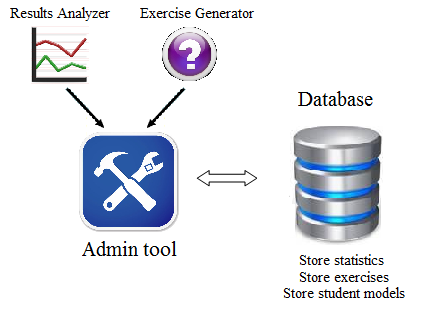
\includegraphics[scale=0.8]{admin_tool_architecture}
\caption{Architecture of the jSCAPE admin tool}
\label{fig:admin_tool_architecture}
\end{figure}

In the rest of this chapter we justify our design choices and discuss the implementation of the various components and features of the jSCAPE system.

\section{Technology choices}
Most software in the area of computer based education is web-based, as demonstrated by the review of related work in chapter \ref{chap:related-work}. We decided to follow this trend, as it makes deployment easier, and because students are usually quite familiar with web browsers. Therefore, the three-tier architecture of web client, server and database was the natural model of choice for creating such a system. There are multiple technologies which can be used to develop the client side. Some of these are HTML5, CSS, Javascript, Flash, and Java applets.\newline

We decided to take the approach of Java applets because we have had a lot of experience with developing large scale programs in this language. In addition, in our opinion, Java applets are better for creating rich web applications which resemble desktop applications. Websites require the user to continuously click links, and load web pages to access a feature, and we think that this model isn't suitable for developing jSCAPE. Finally, implementing jSCAPE as an applet allows it to run in Java web start mode or as a stand alone desktop application, thanks to the Java deployment framework. \newline

However, regular Java applets use the Swing library for GUIs, and as a result, the interface doesn't end up being user-friendly or visually appealing. This is certainly a problem, because although the application can present powerful and useful features, students will only use it if the interface is intuitive and aesthetically pleasing\cite{Interface-study}. \newline

This realisation led us to researching libraries which could improve the interfaces of Java applets, and discovering JavaFX. JavaFX is intended as a replacement for the Swing GUI library, and is designed to provide a lightweight, hardware-accelerated Java UI platform for creating rich internet applications\cite{JavaFX}. The JavaFX library includes a powerful and visually appealing statistics package, with support for pie charts, bar charts, line charts, scatter charts, tables, etc... which was more than enough to implement the statistics tracking and displaying component of jSCAPE. In addition, this would allow us to easily add more displayable statistics in the future (section \ref{sec:future-work}), if required. \newline

JavaFX also provides the functionality of embedding a \textsf{WebView}, a browser component which supports HTML5, CSS and Javascript, into the applet. We found that this could be an interesting feature to use for developing exercises with variety and interactivity, For instance, this component is used in the Binary Tree exercises to display the binary trees (section 5.??). \newline

Every web application needs some sort of server to handle web client requests. We looked at Java Server Pages (JSP) and Java Servlets, but the setup and organization required to make them work seemed to be too much work for the very little advantages they offered. Instead we opted to write our own Java server because this would offer more control for handling requests and more flexibility for extensions in the future. In addition, the time and amount of code required to write a functional server was very minimal. Indeed, the basic components of our custom built server fit into approximately 300 lines of code. \newline

A database is needed for permanent storage of the system's state, student models, exercises, etc... Thus, to do this, we use a PostgreSQL database and connect to it using the associated Java Database Connectivity (JDBC) driver. \newline

Throughout this chapter, we will give more detail about which tables are maintained by the system, and how they are used. In addition, we will introduce some other technologies and libraries used in this project later on, when we look at the exercise generation and display processes.
\section{Design}
This section describes the design of the jSCAPE system.

\subsection{Client}
\begin{figure}[H]
\centering
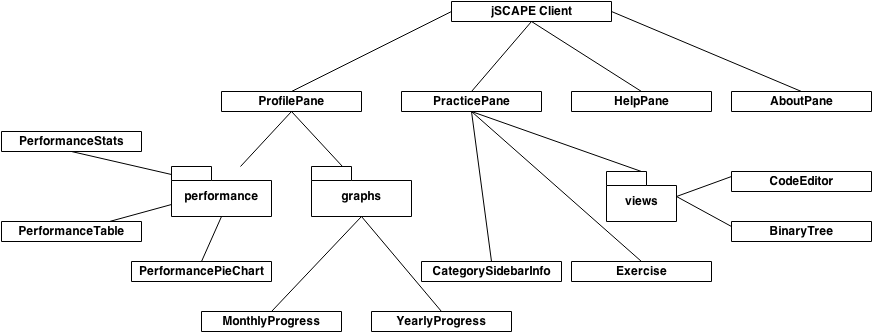
\includegraphics[width=\textwidth,height=\textheight,keepaspectratio]{class_diagram_client}
\caption{Class diagram of the jSCAPE client.}
\label{fig:class_diagram_client}
\end{figure}

Figure \ref{fig:class_diagram_client} shows the class diagram of the jSCAPE client, which is what is embedded into the web browser, and displayed to students. We briefly describe the classes:
\begin{itemize}
\item \textsf{ProfilePane}: The Profile tab of the application.
      \begin{itemize}
      \item[-] \textsf{performance} package:
               \begin{itemize}
               \item[-] \textsf{PerformanceStats}: Stores performance statistics, i.e. exercise category, correct answers, wrong answers.
               \item[-] \textsf{PerformanceTable}: Table wrapper to display \textsf{PerformanceStats} objects.
               \item[-] \textsf{PerformancePieChart}: PieChart wrapper to display \textsf{PerformanceStats} objects.
               \end{itemize}
      \item[-] \textsf{graphs} package:
               \begin{itemize}
               \item[-] \textsf{MonthlyProgress}: StackedBarChart wrapper to display monthly progress statistics.
               \item[-] \textsf{YearlyProgress}: StackedBarChart wrapper to display yearly progress statistics.
               \end{itemize}
      \end{itemize}
\item \textsf{PracticePane}: The Practice tab of the application.
       \begin{itemize}
       \item[-] \textsf{Exercise}: Stores an exercise and information such as exercise ID, description, choices, solution, display values.
       \item[-] \textsf{CategorySidebarInfo}: Stores information to create the sidebar of an exercise window.
       \item[-] \textsf{views} package contains the classes to render exercises in the left part of the Practice tab:
                \begin{itemize}
                \item[-] \textsf{BinaryTree}: Component capable of drawing binary trees.
                \item[-] \textsf{CodeEditor}: Component capable of displaying programming code in a code editor.
                \end{itemize}
       \end{itemize}

\item \textsf{HelpPane}: The Help tab of the application, displays the manual.

\item \textsf{AboutPane}: The About tab of the application, displays information about what the application does.
\end{itemize}

The jSCAPE client accounts for approximately 2500 lines of code.

\subsection{Server}
\begin{figure}[H]
\centering
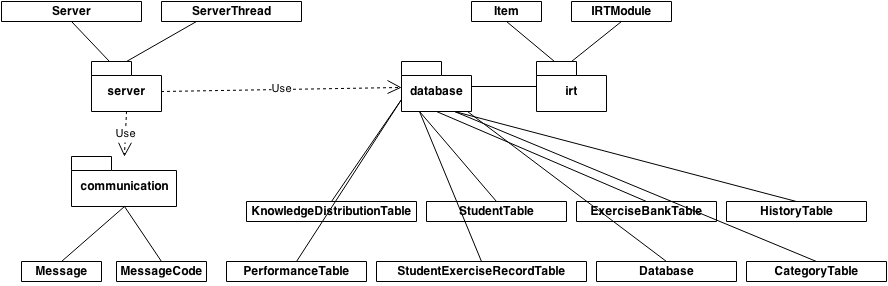
\includegraphics[width=\textwidth,height=\textheight,keepaspectratio]{class_diagram_server}
\caption{Class diagram of the jSCAPE server.}
\label{fig:class_diagram_server}
\end{figure}

Figure \ref{fig:class_diagram_server} shows the class diagram of the jSCAPE server, and the database classes the server uses to satisfy client requests. We briefly describe the classes:
\begin{itemize}
\item \textsf{server} package:
      \begin{itemize}
      \item[-] \textsf{Server}: The server, creates \textsf{ServerThread}s to handle client connections.
      \item[-] \textsf{ServerThread}: Receives requests from the client(s), performs work and replies to the client(s).
      \end{itemize}
\item \textsf{communication} package:
      \begin{itemize}
      \item[-] \textsf{Message}: A data structure to hold information. This is the unit which ``travels" between the client and server, and vice-versa.
      \item[-] \textsf{MessageCode}: Enum to identify structure and format of a \textsf{Message}.
      \end{itemize}     
\item \textsf{database} package:
      \begin{itemize}
      \item[-] \textsf{Database}: Manages the connection info and hands out connections to the components that wish to access the physical database.
      \item[-] \textsf{StudentTable}: Stores profile information of students, login names, passwords, etc...
      \item[-] \textsf{CategoryTable}: Stores the exercise categories, their description and associated lecture notes or helpful website links.
      \item[-] \textsf{PerformanceTable}: Stores performance statistics, such as correct answers and wrong answers, of students for the different exercise categories.
      \item[-] \textsf{HistoryTable}: Stores performance statistics of students for each day they used the system.
      \item[-] \textsf{ExerciseBankTable}: Stores the exercises, some exercise metrics and difficulty parameters.
      \item[-] \textsf{StudentExerciseRecordTable}: Stores which exercises students have answered and whether they got it correct or incorrect.
      \item[-] \textsf{KnowledgeDistributionTable}: Stores the knowledge distribution of the student per exercise category, in the case that Item Response Theory is used.
      \end{itemize}
\item \textsf{irt} package: This package is a Java implementation of Item Response Theory.
      \begin{itemize}
      \item[-] \textsf{Item}: An IRT item, which stores an exercise ID and item parameters.
      \item[-] \textsf{IRTModule}: Implements IRT concepts such as the item response function, the item information function, ability estimation, etc...
      \end{itemize}
\end{itemize}

\subsection{Exercises and exercise generators}
\label{subsec:exercises-and-exercise-generators}
\begin{figure}[H]
\centering
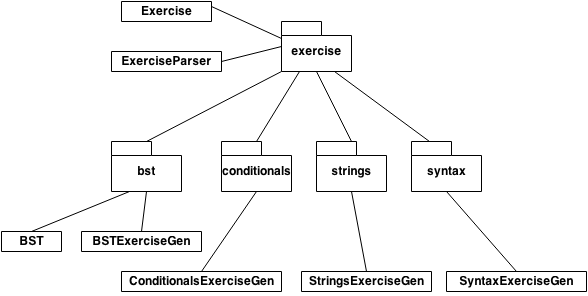
\includegraphics[width=\textwidth,height=\textheight,keepaspectratio]{class_diagram_exercises}
\caption{Class diagram of the currently implemented exercise generators.}
\label{fig:class_diagram_exercises}
\end{figure}

Figure \ref{fig:class_diagram_exercises} shows the class diagram for exercises and the implemented exercise generators, at the time of writing this report. We briefly describe the classes:
\begin{itemize}
\item \textsf{Exercise}: Stores an exercise and information such as exercise ID, description, choices, solution, display values.
\item \textsf{ExerciseParser}: Special XML parser to decode the exercise format and return an \textsf{Exercise}.
\item \textsf{bst} package:
      \begin{itemize}
      \item[-] \textsf{BST}: Java implementation of binary trees with standard functions such as insert, traversal, height, etc...
      \item[-] \textsf{BSTExerciseGen}: Generates an exercise for the Binary Tree exercise category.
      \end{itemize}
\item \textsf{conditionals} package:
      \begin{itemize}
      \item[-] \textsf{ConditionalsExerciseGen}: Generates an exercise for the Conditionals exercise category.
      \end{itemize}
\item \textsf{strings} package:
      \begin{itemize}
      \item[-] \textsf{StringsExerciseGen}: Generates an exercise for the Strings exercise category.
      \end{itemize}
\item \textsf{syntax} package:
      \begin{itemize}
      \item[-] \textsf{SyntaxExerciseGen}: Generates an exercise for the Syntax exercise category.
      \end{itemize}                 
\end{itemize}

The exercise and exercise generators account for approximately 2400 lines of code.

\subsection{Admin tool}
We won't go into the details of the admin tool design. Essentially it reuses classes from other components and adds a few modifications.\newline

This component accounts for approximately 2000 lines of code, although most of those lines are copied from other components.

\section{Server and client-server communication}
The server is responsible for servicing all client requests, for instance, requesting performance statistics or requesting a new exercise. It is custom built, multithreaded and written in pure Java, using Sockets and Object input/output streams. The basic server class and the mechanism to communicate with clients accounts for approximately 300 lines of code. \newline

\lstinputlisting[language=Java, caption={Serializable message object used for client-server communication.}, label={lst:message.java}]{\listings/message.java}
The code in \ref{lst:message.java} shows the basic unit that travels between the client and the server, and vice-versa. A message consists of a message code, used to determine its structure, and a payload of request parameters, in the form of an \textsf{ArrayList$<$String$>$}.\newline

The existing message request codes are shown in \ref{lst:message_codes.java}. The server uses these to determine what the client has requested, how the request message is formatted and which actions to perform to service the request. \newpage

\lstinputlisting[language=Java, caption={Message request codes.}, label={lst:message_codes.java}]{\listings/message_codes.java}

The code snippet in \ref{lst:example_service.java} gives an example of how the client can construct a request. In this particular example the client is requesting the statistical data about the student's performance. On line 1, a \textsf{Service} is created. A \textsf{Service} is a task that can be performed over and over again by calling the \textsf{restart()} method, like on line 12. Lines 2 to 10 determine what the service should do when it is started. Lines 4 and 5 add the student's login name as a request parameter. On lines 6 and 7, the message is constructed with the appropriate message code, and the request parameters. On line 9, the message is sent to the server, and the reply from the server is stored in the \textsf{Service}, for the client to use later on.\newline

\lstinputlisting[language=Java, caption={An example client request.}, label={lst:example_service.java}]{\listings/example_service.java}

In addition to communicating with the client, the server also communicates with the PostgreSQL database. This is to retrieve the data requested by the client, and to update the state of the system as the student answers exercises, for instance. Therefore, a database module was created with methods to perform the necessary functions. \newline

\lstinputlisting[language=Java, caption={An example database retrieval method.}, label={lst:example_database_method.java}]{\listings/example_database_method.java}

In listing \ref{lst:example_database_method.java} we give an example of a database retrieval method. Such methods form a large part of the database module. All methods which read from the database return a \textsf{ArrayList$<$String$>$}, so that this can be immediately put in the reply message from the server to the client. In this particular example, the method retrieves performance statistics for the student identified by \textsf{loginName}. Line 6 creates the data structure to hold the information which will be read from the database. Lines 8 to 18 create the query, and send it to the database to be executed. In lines 20 to 24, the result of the query is added to the data structure. Finally, on line 27, all this information is returned to the server, which can now encapsulate this in a reply message, and send that to the client.\newline

The database module also includes methods to update the information stored in the database. These methods simply execute an SQL \textsf{UPDATE} query, and return no status value. \newline

This database module is also used by the jSCAPE admin tool to analyze results and manage the exercise bank. The module comprises of 8 classes, one main database class and one for each database table, and accounts for approximately 1500 lines of code.

\section{Implementing Computerized Adaptive Testing (CAT)}
\label{sec:implementing-cat}
We refer back to the background chapter, section \ref{sec:CAT}, where we outlined the components necessary to build a CAT. We also base this section on the work of SIETTE, for the reasons outlined in the related work chapter, section \ref{sec:SIETTE}.\newline

We decide to follow many of the implementation details of SIETTE, that is, to use the Bayesian estimation method, with a knowledge distribution consisting of 11 discrete knowledge levels, ranging from 0 to 10. In addition, the exercise selection algorithms used by jSCAPE will be presented. We now give more details about how the different CAT components are implemented in jSCAPE.

\subsection{Calibrated item pool}
We mentioned in section \ref{sec:CAT}, that calibration was a complex process, and that to be done accurately it required a considerable amount of data. However,  to obtain this data we would need to have hundreds of students answer jSCAPE exercises and record whether they got the right or wrong answer. Even if this data could be obtained, calibrating the exercises would then require to purchase specialized software. \newline

Therefore, to show what jSCAPE would be capable of, given an accurately calibrated item pool, we require teachers to input item parameters, just as in SIETTE. In the case of a multiple choice question, the pseudo-chance parameter, $c$, will be equal to $0.25$. The difficulty parameter, $b$, takes discrete values between 0 and 11, and the discrimination parameter, $a$, takes values between $0.5$ and $1.5$. \newline

Evidently, this won't end up being as accurate as an item pool where the calibration process was based on thousands of responses to exercises, but it is the best we can do given the circumstances.

\subsection{Starting point}
The starting point refers to the state of the system when no exercises have been administered to a student. In jSCAPE, no prior information about students is known, so the system's initial ability estimate for the student corresponds to the mean on the ability scale, i.e. $\theta = 5$. In addition, the initial knowledge distribution will be a uniform distribution with $P(\theta)=\frac{1}{11}$, where $P(\theta)$ is the probability that the student's knowledge level is equal to $\theta$. These initial assumptions are taken for every exercise category.

\subsection{Implementing exercise selection algorithms}
\label{subsec:implementing-exercise-selection-algorithms}
In this section we discuss the exercise selection algorithms which have been implemented in jSCAPE. We go through these in chronological order of implementation. In the final jSCAPE system, all these selection algorithms are still present, allowing the teacher to choose which procedure to use for administering exercises to students.

\subsubsection{Random selection}
Random selection was the first ``algorithm" implemented. It allowed us to test the system and put everything in place to then develop the more sophisticated algorithms which will follow. This algorithm is quite simple, it picks an exercise at random from the exercises that haven't been answered yet by a student.

\subsubsection{Selecting based on the difficulty category}
The idea for the next selection algorithm arose after coming across PAT (section \ref{sec:PAT}), software used for assessing Greek high school students' programming knowledge.\newline

We decide to define difficulty categories for exercises. Category A is for easy exercises, category B is for intermediate exercises and category C is for difficult exercises. When an exercise is added manually to the exercise bank, the teacher can choose which difficulty category the exercise belongs to. In section \ref{subsec:exercise-generation}, we show some mechanisms which enable the exercise generators to determine an exercise's difficulty category, based on some simple metrics.

\begin{figure}[H]
\centering
\begin{tikzpicture}[>=stealth',shorten >=1pt,auto,node distance=3cm]
  \node[initial,state] (A1)      {$A1$};
  \node[state]         (A2) [right of=A1]  {$A2$};
  \node[state]         (A3) [right of=A2] {$A3$};
  \node[state]         (B1) [below of=A3] {$B1$};
  \node[state]         (B2) [left of=B1] {$B2$};
  \node[state]         (B3) [left of=B2] {$B3$};
  \node[state]         (C1) [below of=B3] {$C1$};
  \node[state]         (C2) [right of=C1] {$C2$};
  \node[state]         (C3) [right of=C2] {$C3$};


  \path[->] (A1)  edge [loop above] node {wrong} (A1)
             edge [bend left] node {correct} (A2)
        (A2) edge [bend left]  node {wrong} (A1)
             edge [bend left] node {correct} (A3)
        (A3) edge [bend left]  node {wrong} (A2)
             edge [bend left] node {correct} (B1)
        (B1) edge [bend left]  node {wrong} (A3)
             edge [bend left] node {correct} (B2)
        (B2) edge [bend left]  node {wrong} (B1)
             edge [bend left] node {correct} (B3)
        (B3) edge [bend left] node {wrong} (B2)
             edge [bend left] node {correct} (C1)
        (C1) edge [bend left] node {wrong} (B3)
             edge [bend left] node {correct} (C2)
        (C2) edge [bend left] node {wrong} (C1)
             edge [bend left] node {correct} (C3)
        (C3) edge [loop above] node {correct} (C3)
             edge [bend left] node {wrong} (C2);             
\end{tikzpicture}
\caption{State machine of adaptive difficulty categories.}
\label{state-machine}
\end{figure}

Figure \ref{state-machine} shows the state machine implemented by this exercise selection algorithm. For every exercise category, initially students will be presented with exercises from the A difficulty category. A correct answer gets the student closer to getting promoted to a harder difficulty category, for that particular exercise category only. On the other hand, a wrong answer gets the student closer to getting demoted to an easier difficulty category. When a student changes exercise category, or leaves jSCAPE, this difficulty category is saved so that exercises of the appropriate difficulty can be selected during the next session. \newline

The algorithm implemented in jSCAPE waits a while to confirm that the student is in fact ready to move to the next difficulty category. Similarly, the algorithm waits a while before decreasing the difficulty, to account for careless slip ups. For these reasons, we think that the algorithm in jSCAPE is better than the one implemented in PAT. \newpage

\subsubsection{Selecting using Item Response Theory}
This algorithm is the most sophisticated exercise selection algorithm and it is based on the concepts of Item Response Theory. \newline

\lstinputlisting[language=Java, caption={An item.}, label={lst:item.java}]{\listings/item.java}

First of all, we define an item as shown in listing \ref{lst:item.java}. The \textsf{itemID} is an identifier which points to an exercise in the exercise bank. The variables \textsf{a}, \textsf{b} and \textsf{c} refer to the item parameters $a$, $b$ and $c$. These are also columns in the exercise bank database table, null values indicate that the exercise isn't an IRT exercise. \newline

For item selection, we use the maximum information method, which consists in choosing the item with the maximum amount of information for the student's current ability estimate. \newline

\lstinputlisting[language=Java, caption={Item information algorithm.}, label={lst:item_information.java}]{\listings/item_information.java}

In listing \ref{lst:item_information.java} we show the method which computes item information for a given item.

\lstinputlisting[language=Java, label={lst:max_item_information.java}, caption={Maximum information method.}]{\listings/max_item_information.java}

In listing \ref{lst:max_item_information.java} we show the maximum information method, which takes a list of items and the current ability estimate for a student. The algorithm then searches the items for the item with the maximum amount of information, and returns the index of that item in the list, so that it can be presented to the student. \newline

Normally, \textsf{itemList} would be all the exercises that a student hasn't answered yet, for a particular exercise category. However, this can be optimized to include only those exercises whose difficulty parameter is of distance 1 from the current ability estimate for that student. Another possible improvement would be to implement the item information function and maximum information method directly into the database, as user defined functions.\newline

A simulation of jSCAPE in IRT mode is included in appendix \ref{chap:irt-simulation}. Amongst other things, it shows how the items which are selected are those which maximize item information.

\subsection{Scoring algorithm}
The scoring algorithm refers to the steps taken to update the student's ability estimate after an exercise has been answered. We decide to use the Bayesian estimation method for this, just as in SIETTE. If an exercise with an assigned difficulty category is answered, then none of the following is done.
\newpage

\lstinputlisting[language=Java, label={lst:item_response_function.java}, caption={Item response function (3PL).}]{\listings/item_response_function.java}

First, we list the Java implementation of the 3PL item response function in listing \ref{lst:item_response_function.java}. This corresponds to the probability of answering \textsf{item} correctly, given \textsf{thetaEstimate} as the current ability estimate for the student. \newline

Recall, that the Bayesian estimation method computes the posterior knowledge distribution from the prior knowledge distribution and observed data in the student's answer to an exercise.

\begin{equation}
\label{eq:compute-posterior}
P(\theta=k|u_i) = \frac{P(u_i|\theta=k)P(\theta=k)}{\sum_{j=0}^{10}P(u_i|\theta=j)P(\theta=j)}, \;\;\;\;\;\;\;\;\; \text{for each } k=0 \text{ to } k=10 
\end{equation}

Equation \eqref{eq:compute-posterior} shows how jSCAPE computes the posterior distribution, after a student has answered exercise $i$, with $u_i=1$ if he answered correctly, and $u_i=0$ otherwise. $P(u_i|\theta=k)$ is the item response function for item $i$, and $P(\theta=k)$ is the prior knowledge distribution. We apply Bayes' theorem using these two pieces of information to compute the new knowledge distribution. \newline

The implementation of the scoring algorithm, that is, the item response function, the computation of the posterior distribution, etc... forms part of the Item response theory module. It contains quite a few lines of code, thus we include it in appendix \ref{chap:irt-module}.\newline

A simulation of jSCAPE in IRT mode is included in appendix \ref{chap:irt-simulation}. Amongst other things, it shows how the knowledge distribution is updated after a student has answered an exercise.

\subsection{Termination criterion}
When discussing CATs, we mentioned the need for a termination criterion. However, for jSCAPE we wanted no limit to be imposed on the number of exercises a student could answer. As long as exercises are available in the exercise bank, and as long as a student wants to practice, then he will be able to do so. The only termination criterion per say, is when a student exits an exercise category to practice exercises of another category. This means that when a student goes back to that previous exercise category, his knowledge distribution will continue to evolve from where it left off. A teacher could, for instance, reset the knowledge distribution every week or month to get more accurate and recent estimates of a student's knowledge.

%talk about Beanshell for ex gen
\section{Exercises}
\label{sec:exercises-implementation}
The possibility to practice understanding of programming concepts through exercises can be considered jSCAPE's central feature. In this section we discuss some of the design considerations for exercises, how they are implemented in jSCAPE and how exercise generators can be written to automatically generate these exercises.

\subsection{Design choices}
With jSCAPE's flexible exercise format (section \ref{subsec:jscape-exercise-format}), it is possible to handle multiple types of exercise. However, instead of trying to include a large variety of exercise types, we decide to refine our focus. Therefore, we come up with the following exercise specification:
\begin{itemize}
\item To illustrate the capabilities of jSCAPE, and to introduce variety in the exercises, we decide to define exercises which use different views (e.g. \textsf{BinaryTree}, \textsf{CodeEditor}). Research\cite{Lister} has shown that a code snippet and an exercise asking for the behaviour of the code, provides effective assessment on a student's understanding of code semantics. Therefore, jSCAPE will include this type of exercise, as well as other exercises which don't display a piece of code, for variety purposes, as mentioned before.
\item For those exercises which display code snippets, the code will be written in the Java programming language. However, we note that jSCAPE is language independent and that exercises with code snippets from other languages can easily be supported. This is in fact a possible extension to the system (section \ref{sec:future-work}).
\item Exercises won't ask students to write any code, because students usually have other assignments which ask them to do so. jSCAPE exercises are intended to practice understanding of fundamentals and to reinforce mental models of what programming language constructs actually do. In addition, this would require jSCAPE to include a component for checking the style and correctness of code written by students. Writing this component would take time off implementing the other components and features of jSCAPE.
\item Feedback to an exercise will only be very basic: indicating whether the student got the exercise right or wrong, and displaying the solution. Feedback will be shown immediately after the student has answered the exercise, because evidence\cite{Mitrovic} suggests that this is the most effective way for providing feedback. More advanced feedback is a possible extension to the system (section \ref{sec:future-work}).
\item Exercises will be multiple choice only, so that the three-parameter logistic (3PL) model of Item Reponse Theory can be used to implement adaptive difficulty.
\end{itemize}

\subsection{jSCAPE exercise format}
\label{subsec:jscape-exercise-format}
To represent an exercise entity, jSCAPE uses a simple XML tagged document. This is shown in listing \ref{lst:exercise_format}.\newline

\lstinputlisting[language={xml}, tabsize=4, caption={Exercise format.},label={lst:exercise_format}]{\listings/exercise_format.xml}

To understand the format, recall how exercises are displayed to students in the Practice tab (section \ref{subsec:pratising-programming}). Exercise data is shown in the left window, and the exercise description and choices are shown in the right window.
We now explain the significance of these tags:
\begin{itemize}
\item The first \textsf{$<$display$>$} tag encloses information about the left window. The enclosed \textsf{$<$view$>$} tag corresponds to the component required to render the exercise data in the left window. Currently, two values are possible for this tag, \textsf{BinaryTree} and \textsf{CodeEditor}. The enclosed \textsf{$<$value$>$} tag holds the data that is passed to the rendering component to be rendered accordingly.
\item The second \textsf{$<$display$>$} tag encloses information about the right window. The enclosed \textsf{$<$view$>$} tag corresponds to the type of exercise, and currently only one value is possible, \textsf{Multiple Choice}. The enclosed \textsf{$<$value$>$} tag holds the exercise description, i.e. the question asked. The \textsf{$<$choice$>$} tags correspond to the possible choices given to the student, and finally, the \textsf{$<$solution$>$} tag contains the solution to the exercise.
\item The last \textsf{$<$display$>$} tag encloses a \textsf{$<$difficulty$>$} tag which gives the difficulty category of the exercise. Details about the difficulty category parameter will be given in the next section, on exercise generation.
\end{itemize}

Some examples of jSCAPE exercises are shown in appendix \ref{chap:example-jscape-exercises}.

\subsection{Exercise generation}
\label{subsec:exercise-generation}
Although jSCAPE allows for exercises to be added manually, this isn't a feasible way to build a large exercise bank. Therefore, we introduce the process of exercise generation, and give details as to how we implemented exercise generators for some exercises. In simple terms, exercise generation requires filling the tags of the jSCAPE exercise format. In this subsection, we will focus on the exercise generators for two exercise categories: Binary Trees and Conditionals. The other exercise generators are implemented in the same fashion.

\subsubsection{Binary Tree exercise generation}
Recall the class diagram for exercises and exercise generators (section \ref{subsec:exercises-and-exercise-generators}). The exercise generator for Binary Tree exercises is called \textsf{BSTExerciseGen}, and uses \textsf{BST}, a Java implementation of binary trees, to help in generating exercises. An example Binary Tree exercise, in the jSCAPE exercise format, is shown in appendix \ref{chap:example-jscape-exercises}.\newline

The first step to generating a Binary Tree exercise is selecting the appropriate view for the left window. For this exercise category, we take as an example the creation of exercises which display binary trees as exercise data, and a question that asks what will be printed for various traversal orders. Therefore, we use the \textsf{BinaryTree} view, and this goes into the \textsf{$<$view$>$} tag of the first \textsf{$<$display$>$} tag, as shown in listing \ref{lst:binary_tree_gen1.java}.\newline

\lstinputlisting[language={java}, caption={First part of exercise generation.},label={lst:binary_tree_gen1.java}]{\listings/binary_tree_gen1.java}

Next, \textsf{BST} generates a binary tree in Java, from a set of random numbers. This binary tree is either balanced with probability $\frac{2}{3}$ or left unbalanced with probability $\frac{1}{3}$. Our reasoning for this is that students will probably be more familiar with balanced binary trees, therefore unbalanced binary trees can be left for exercises of greater difficulty.\newline

The \textsf{BinaryTree} view is implemented using the JavaScript InfoVis Toolkit (JIT)\cite{JIT}. This library provides tools for creating interactive visualizations for the web, and requires displayable data to be in the JSON format. Therefore, \textsf{BSTExerciseGen} converts the Java binary tree into the JSON format accepted by the \textsf{BinaryTree} view, and this goes into the \textsf{$<$value$>$} tag of the first \textsf{$<$display$>$} tag. This process is illustrated below. \newline

\begin{lstlisting}[language={Java}, label={lst:binary_tree_gen2.java}]
BST<Integer> bst = createBST(randomNumbers);
xmlExercise += bst.toJSON();
                            
\end{lstlisting}

Figure \ref{fig:binary_tree_example} shows an example binary tree and listing \ref{lst:binary_tree_json} is the JSON representation of that binary tree. 

\begin{figure}[H]
\centering
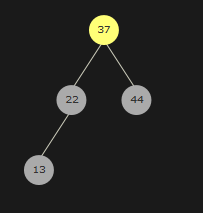
\includegraphics[scale=0.9]{binary_tree_example}
\caption{A binary tree.}
\label{fig:binary_tree_example}
\end{figure}

\lstinputlisting[language={json}, tabsize=4, caption={JSON representation of the binary tree in figure \ref{fig:binary_tree_example}.},label={lst:binary_tree_json}]{\listings/binary_tree_json.json}

\newpage

Next, we create a data structure with the results of all the traversal orders. This is shuffled and used to complete the \textsf{$<$choice$>$} tags. We select a traversal order, at random, from the possible traversal orders, i.e. pre, in, post and level order. This traversal order is inserted into the question, and the result of that traversal is inserted into the \textsf{$<$solution$>$} tag. This step is illustrated in listing \ref{lst:binary_tree_gen2.java}. \newline

\lstinputlisting[language={java}, caption={Generating question and choices.},label={lst:binary_tree_gen2.java}]{\listings/binary_tree_gen2.java}

For the \textsf{$<$difficulty$>$} tag, recall that we have three difficulty categories, A, B and C. We will assign a difficulty category based on some simple metrics. We decide not to use item response theory for automatically generated exercises because any estimation the exercise generator would make for the $a$ and $b$ parameters would be terribly inaccurate.\newline

For this exercise category, we assume that the size, the height and whether the tree is balanced or not, can impact the difficulty of the exercise. For instance, when the number of nodes is less than 7, we assign the exercise to difficulty category A, between 7 and 12 nodes, to difficulty category B and more than 12 nodes to difficulty category C.

\subsubsection{Conditionals exercise generation}

\section{Collecting statistical data}
One of the main features of jSCAPE is tracking student progress through statistical data. In this section we briefly look at what statistical data is collected and how it is organized in the database.

\begin{figure}[H]
\centering
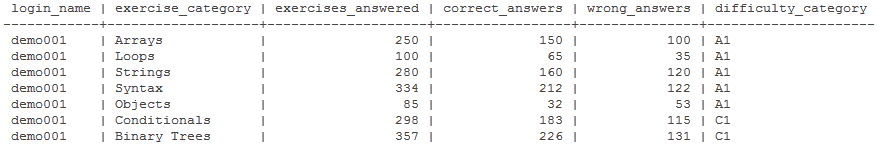
\includegraphics[width=\textwidth,height=\textheight,keepaspectratio]{performance_database_table}
\caption{Performance database table.}
\label{fig:performance_database_table}
\end{figure}

Figure \ref{fig:performance_database_table} shows that, for every student, the system records the number of exercises answered, the number of correct answers and the number of wrong answers for each exercise category defined by the teacher. In addition, the system keeps track of what difficulty category the student has reached for every exercise category. This is the information that gets displayed in the pie charts and performance table.

\begin{figure}[H]
\centering
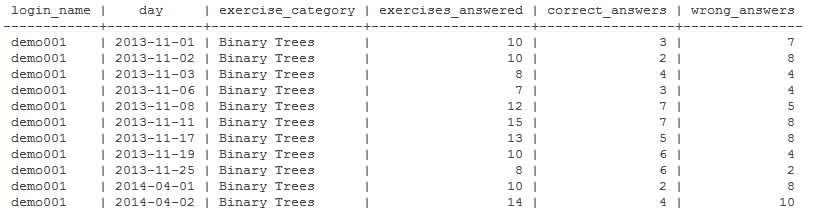
\includegraphics[width=\textwidth,height=\textheight,keepaspectratio]{history_database_table}
\caption{History database table.}
\label{fig:history_database_table}
\end{figure}

Figure \ref{fig:history_database_table} shows that the system records, for every student, the days where exercises were answered, the number of exercises answered answered on that day, the number of correct answers and the number of wrong answers, for every exercise category. This data is used to plot the stacked bar charts of monthly and yearly progress.

\begin{figure}[H]
\centering
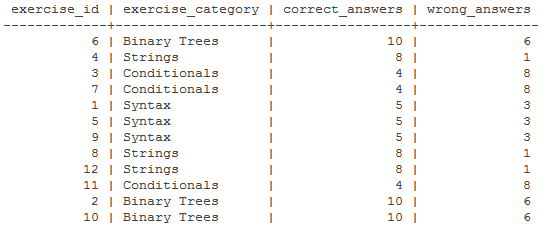
\includegraphics[width=\textwidth,height=\textheight,keepaspectratio]{exercisebank_database_table}
\caption{Exercise bank database table.}
\label{fig:exercisebank_database_table}
\end{figure}

Figure \ref{fig:exercisebank_database_table} shows that the system records the number of correct answers and wrong answers for each exercise. This is a useful feature for teachers to identify trends in which type of exercises students are having trouble with and which type of exercises students are having little trouble answering correctly.

\section{Summary}
In this section, we gave details of the design and implementation of jSCAPE.\newline

We started off by justifying the different technologies we used in the project. We then showed the design of the system and its various components through class diagrams and explanations.\newline

Next, we looked at how computerized adaptive testing was implemented in jSCAPE. More specifically, we mentioned that it is possible to choose between random, difficulty category based and IRT based exercise selection algorithms. \newline

We then talked about the types of exercises available in jSCAPE, the exercise format and we showed how exercise generators could be coded to generate exercises automatically.\newline

Finally, we briefly discussed how jSCAPE collected statistical data by maintaining several database tables with various statistics on exercises, student performance and system usage.
